\documentclass[conference]{IEEEtran}
\usepackage[utf8]{inputenc}
\usepackage{amsmath,amssymb}
\usepackage{booktabs}
\usepackage{graphicx}
\usepackage{cite}
\usepackage{textcomp}
\renewcommand{\arraystretch}{0.88}
\raggedbottom
\setlength{\textfloatsep}{4pt plus 2pt minus 2pt}
\setlength{\floatsep}{3pt plus 1pt minus 1pt}
\setlength{\intextsep}{4pt plus 2pt minus 2pt}

\title{When Super-Resolution Hurts: A Controlled Study of Ear-Based Gender Classification under Deployment Constraints}

\author{
\IEEEauthorblockN{
Thai Le Quang\textsuperscript{a,b}, Huy Nguyen Quoc\textsuperscript{a}, Dzi Lam Tran Tuan\textsuperscript{a}, Vinh Truong Hoang\textsuperscript{a,*}
}
\IEEEauthorblockA{
\textsuperscript{a}Faculty of Information Technology, Ho Chi Minh City Open University, Ho Chi Minh City, Vietnam\\
\textsuperscript{b}Faculty of Data Science in Business, Ho Chi Minh University of Banking,
Ho Chi Minh City, Vietnam\\
*Corresponding author: vinh.th@ou.edu.vn
}
}

\begin{document}

\maketitle

\begin{abstract}
Engineers deploying an ear-based gender classifier on unconstrained images must decide whether to place a super-resolution model in front of it. Earlier comparisons on EarVN1.0 cannot inform this decision because they are confounded in two ways: super-resolution inputs were evaluated with a different training recipe, and image-level splits leak subject identity. We train each of six backbones once on Original images and evaluate that same checkpoint on Original, Bicubic, Real-ESRGAN, and SwinIR inputs over five subject-disjoint folds. Real-ESRGAN and SwinIR reduce accuracy by 3.2 and 3.0 points on average, while Bicubic leaves it unchanged. The loss is concentrated in crops below 128 pixels and comes with a systematic shift of the decision toward the female class: male recall drops by about 7 points for every backbone. Retraining the recognizer on each super-resolution variant recovers Original accuracy in all eighteen model-variant combinations, and the pooled gap is equivalent to zero within one point, which points to a recoverable distribution shift. Without retraining, recalibrating the decision threshold or the batch-normalization statistics on unlabeled super-resolution images recovers 56--79\% of the loss. These results yield an evidence-based decision rule: do not insert off-the-shelf super-resolution before a fixed classifier; if super-resolution is required, recalibrate on unlabeled super-resolution images; if retraining is possible, train and deploy on Original images.
\end{abstract}

\begin{IEEEkeywords}
Decision support, ear biometrics, gender classification, super-resolution, test-time adaptation
\end{IEEEkeywords}

\section{Introduction}
Ear crops can be taken from headshots, full-body images, or video without the subject facing the camera, which makes the ear a useful non-contact cue for soft biometrics such as gender~\cite{emersic2017,pflug2012}. Earlier ear-based gender recognition used three-dimensional shape~\cite{lei2013} and two-dimensional sparse coding~\cite{khorsandi2013}; on EarVN1.0, deep networks outperform hand-crafted descriptors and reach 91.12\% with VGG19~\cite{vgg} under a random image-level split~\cite{nguyenquoc2020}.

Because EarVN1.0~\cite{hoang2019earvn} images are cropped from unconstrained photos, native resolution varies from a few dozen to several hundred pixels on a side. A natural question is whether a generic super-resolution (SR) model placed before the classifier improves gender prediction. In our own preliminary runs, however, switching to Real-ESRGAN~\cite{realesrgan} or SwinIR~\cite{swinir} was accompanied by a change from SGDM with zero weight decay to AdamW with weight decay, so a higher score after such ``SR training'' may reflect the better recipe, not the SR input. Image-level splits can also leak subject identity through near-duplicate crops, which inflates absolute accuracy. We therefore ask a narrower question: with the recognizer, optimizer, checkpoint, split, and final input geometry held fixed, does generic SR help or hurt ear-based gender classification compared with the original crop and with bicubic upsampling? And if it hurts, can the loss be recovered by retraining the recognizer on SR images?

The recognizer is trained on Original images only, and the identical checkpoint is evaluated on Original, Bicubic, Real-ESRGAN, and SwinIR inputs. A subject-disjoint protocol is our main setting; a legacy image-level split is kept for comparison with prior work. A second, matched-domain protocol retrains the recognizer on each variant under the same locked configuration. For an engineer maintaining a deployed biometric pipeline, the question is a decision with three options: insert an off-the-shelf SR model before the existing classifier, adapt the classifier to SR inputs, or leave the input unchanged. Our goal is to supply the evidence for that decision. Our contributions are:
\begin{itemize}
\item a same-checkpoint protocol on subject-disjoint folds that separates the SR input from the training recipe, with Bicubic as a resampling-path control;
\item evidence that generic SR lowers accuracy for all six backbones, mainly on crops below 128 pixels, and shifts the decision toward the minority class;
\item matched-domain retraining and label-free adaptation tests showing that the loss is recoverable, summarized as a three-level decision rule for deployment (Section~\ref{sec:discussion}).
\end{itemize}
The rest of the paper is organized as follows. Section~\ref{sec:related} reviews ear-based gender recognition and super-resolution as a preprocessing step for recognition. Section~\ref{sec:setup} describes the dataset, the two partitioning protocols, the input variants, and the same-checkpoint, matched-domain, and label-free adaptation protocols. Section~\ref{sec:results} reports the preliminary survey, the same-checkpoint benchmark, the comparison of the two protocols, the prediction-flip and native-size analyses, matched-domain retraining, and label-free adaptation. Section~\ref{sec:discussion} interprets these results and derives a deployment rule, and Section~\ref{sec:conclusion} concludes the paper.

\section{Related Work}\label{sec:related}
Ear biometrics has been surveyed for detection, description, and recognition~\cite{emersic2017,pflug2012}, and local texture descriptors have been compared for ear recognition~\cite{hassaballah2019}. Gender recognition from ears has been studied with three-dimensional ear range data~\cite{lei2013} and two-dimensional sparse representation~\cite{khorsandi2013}. Among public resources, EarVN1.0~\cite{hoang2019earvn} remains the closest large in-the-wild benchmark with gender labels; the comparative study of Nguyen-Quoc and Hoang~\cite{nguyenquoc2020} showed that convolutional backbones surpass classical descriptors such as LBP, HOG, LPQ, BSIF, and GIST on this dataset.

Generic blind SR models such as Real-ESRGAN~\cite{realesrgan} and SwinIR~\cite{swinir} are often used to enhance low-resolution probes before recognition. SR has been reported to improve several downstream vision tasks on low-resolution inputs~\cite{dai2016}, but removing degradations before a CNN classifier does not reliably improve accuracy, whereas training on degraded data does~\cite{pei2021}. For face biometrics, SR models with identity priors were proposed because generic restoration need not preserve recognition cues~\cite{grm2020}. For ear identity recognition on UERC, SwinIR underperformed an unprocessed baseline at both $\times$2 and $\times$4, and a CNN-based model gave only marginal gains attributed to a resolution ceiling~\cite{markicevic2023}. We study ear-based gender classification with the recognizer and recipe fixed, and add a matched-domain condition to separate a distribution-shift explanation from information loss.

\section{Experimental Setup}\label{sec:setup}
\subsection{Dataset and protocols}
The EarVN1.0 database~\cite{hoang2019earvn} contains 28{,}412 unconstrained ear images from 164 Asian subjects, 98 male and 66 female, totalling 17{,}571 and 10{,}841 images respectively. Images are cropped from daily and portrait photos under varying illumination, occlusion, pose, and resolution, with native short side ranging from about 13 to 472 pixels. Because a majority classifier that always predicts male already reaches roughly 61.8\% accuracy, we report macro-F1 and balanced accuracy in addition to raw accuracy throughout. We treat the binary gender labels as dataset annotations only; they do not capture the full diversity of gender identity, and our results should not be read as support for unrestricted demographic profiling.

We use two partitioning protocols. Under the legacy image-level protocol, denoted Protocol A and following prior work, images are split randomly into equal training and testing halves, and 10\% of the training half is held out for early stopping; this admits subject overlap through near-duplicate crops, so we use it only to compare with the earlier baseline. Under the subject-disjoint protocol, denoted Protocol B and our main setting, each of the 164 subjects appears in exactly one partition. We use five-fold stratified group cross-validation, with subjects as groups and gender as the stratification variable, and report mean and standard deviation over folds; within each fold, 15\% of the training subjects are held out as a validation split for early stopping. Table~\ref{tab:dataset} summarizes the counts.

\begin{table}[t]
\centering
\caption{Dataset and protocol statistics.}
\label{tab:dataset}
\small
\begin{tabular}{@{}lccc@{}}
\toprule
Protocol & Split & Male img. & Female img. \\
\midrule
A (legacy)   & Train & 8{,}786 & 5{,}420 \\
A (legacy)   & Test  & 8{,}785 & 5{,}421 \\
B (subject)  & Test (mean/fold) & $\approx$3{,}514 & $\approx$2{,}168 \\
\bottomrule
\end{tabular}
\end{table}

\subsection{Input variants and preprocessing}
All input variants share the same final geometry: a bicubic resize that sets the longer side to 224 pixels, black letterbox padding to $224\times224$, and ImageNet normalization. Let $x$ denote a native RGB crop:
\begin{align}
x_{\text{Orig}} &= \text{PadResize224}(x), \\
x_{\text{Bic}}  &= \text{PadResize224}(\text{Bicubic}_{\times4}(x)), \\
x_{\text{RES}}  &= \text{PadResize224}(\text{RealESRGAN}_{\times4}(x)), \\
x_{\text{Swin}} &= \text{PadResize224}(\text{SwinIR}_{\times4}(x)).
\end{align}
We use the public \texttt{RealESRGAN\_x4plus} checkpoint~\cite{realesrgan} and the SwinIR-Large real-world checkpoint~\cite{swinir} trained with a GAN loss at scale~4. SwinIR runs on whole images; Real-ESRGAN uses tiled inference (tile 400, \texttt{fp32}), which only affects the few crops with a side above 400 pixels. Both SR models are frozen. The final resize upsamples most Original crops, but the $\times4$ Bicubic and SR outputs exceed 224 pixels whenever the native longer side is above 56 pixels and are then downsampled. Bicubic therefore follows the same two-step resampling path as SR and serves as its resampling-path control.

\subsection{Evaluation protocols for SR}\label{sec:protocols}
Our primary evaluation is a same-checkpoint protocol. The recognizer is trained on Original training images only, and that identical checkpoint is applied at test time to $\{x_{\text{Orig}}, x_{\text{Bic}}, x_{\text{RES}}, x_{\text{Swin}}\}$. This asks how inserting SR before an existing recognizer changes its predictions, and it makes corrected and corrupted counts and McNemar tests well defined, since all four conditions are scored by the same weights.

In a secondary, matched-domain protocol we retrain the recognizer on each variant and test it on the same variant (Bicubic to Bicubic, Real-ESRGAN to Real-ESRGAN, SwinIR to SwinIR), comparing against the Original-to-Original run. All runs share the locked configuration, so only the input domain changes. This does not measure the effect of inserting SR before a fixed recognizer, but it tests whether the SR domain is learnable, which separates a recoverable distribution shift from a loss of discriminative information.

We also test two label-free ways to adapt the Original-trained checkpoint to SR inputs without retraining, using each fold's validation images without their labels. Threshold recalibration shifts the female-minus-male logit margin so that the fraction of SR inputs predicted female equals the fraction the same checkpoint predicts on the Original versions of those images, a simple prior-shift correction~\cite{saerens2002}. AdaBN re-estimates the BatchNorm statistics on the SR images~\cite{li2018adabn}; it applies to the four backbones with BatchNorm (MobileNetV2, ResNet50, EfficientNet-B0, MaxViT-T).

\subsection{Models, training, and metrics}
We use six backbones: VGG19~\cite{vgg}, MobileNetV2~\cite{mobilenetv2}, ResNet50~\cite{resnet}, EfficientNet-B0~\cite{efficientnet}, Swin-T~\cite{swintransformer}, and MaxViT-T~\cite{maxvit}, spanning classical, efficiency-oriented, and transformer families. Every run starts from torchvision ImageNet-pretrained weights with a new two-way head. One training configuration was selected on Original validation macro-F1 only, via an 8-epoch optimizer, learning-rate, and weight-decay grid on MobileNetV2, ResNet50, and Swin-T (fold 0), and then locked for every run, including every matched-domain run: AdamW, learning rate $10^{-4}$, weight decay $10^{-4}$, batch size 32, up to 100 epochs. The configuration is not claimed to be optimal; it is fixed so that optimization differences cannot be mistaken for an SR effect. Training uses mixed precision and early stopping with a patience of seven epochs on validation macro-F1. We report accuracy, macro-F1, balanced accuracy, and per-class recall as mean $\pm$ standard deviation over the five Protocol~B folds.

\section{Results}\label{sec:results}
\subsection{Preliminary legacy-recipe survey}
Table~\ref{tab:legacy} compares six backbones on the legacy Protocol A split. Each run trains for a fixed 15 epochs and reports the final epoch. The Original column uses SGDM (learning rate $10^{-3}$, no weight decay), while the Real-ESRGAN and SwinIR columns change both the input and the optimizer (AdamW, weight decay $10^{-4}$). MobileNetV2, ResNet50, EfficientNet-B0, and MaxViT-T improve under both SR recipes, while VGG19 drops by about 1.4 points and Swin-T slightly; the mean change is about $+1.2$ points for both SR methods. Because the recipe changes together with the input, these deltas are not evidence of an SR effect; this uncontrolled comparison only motivated the controlled experiments below.

\begin{table}[t]
\centering
\caption{Preliminary legacy-recipe survey on Protocol A (accuracy, \%). SR columns are uncontrolled: they also switch the optimizer to AdamW with weight decay $10^{-4}$.}
\label{tab:legacy}
\small
\begin{tabular}{@{}lrrrr@{}}
\toprule
Model & Orig.+SGDM & RES & $\Delta$ & SwinIR ($\Delta$) \\
\midrule
VGG19            & 94.59 & 93.21 & $-1.38$ & 93.20 ($-1.39$) \\
MobileNetV2      & 93.23 & 95.07 & $+1.84$ & 94.77 ($+1.54$) \\
ResNet50         & 92.74 & 95.56 & $+2.82$ & 95.08 ($+2.33$) \\
EfficientNet-B0  & 93.96 & 95.87 & $+1.91$ & 96.35 ($+2.39$) \\
Swin-T           & 95.37 & 95.19 & $-0.18$ & 94.98 ($-0.39$) \\
MaxViT-T         & 94.01 & 96.39 & $+2.38$ & 96.66 ($+2.65$) \\
\bottomrule
\end{tabular}
\end{table}

\subsection{Main same-checkpoint benchmark}\label{sec:main}
For each backbone we train once on Original images and evaluate that checkpoint on all four inputs (Table~\ref{tab:main}), with $\Delta_{\text{SR}} = \text{Acc}(\text{SR}) - \text{Acc}(\text{Original})$. Bicubic tracks Original almost exactly (mean $-0.03$ points), so the two-step resampling path alone does not hurt. Real-ESRGAN and SwinIR reduce accuracy for every backbone, by 3.23 and 2.99 points on average, and macro-F1 falls by a similar 3.13 and 2.90 points. Balanced accuracy falls less (2.10 and 1.92 points) because the errors are one-sided: male recall drops by 6.9 and 6.5 points while female recall rises by 2.7 and 2.6 points, for all six backbones (per-backbone values in Supplementary Table~S2). SR thus moves the operating point of the decision toward the female class. The shift is largest and least stable for EfficientNet-B0, whose male recall falls from 92.5\% to 68.4\% on one fold, which explains its high cross-fold standard deviation.

\begin{table}[t]
\centering
\caption{Same-checkpoint benchmark (\%): Acc$\pm$std, Protocol B folds. One checkpoint per model, trained on Original, tested on four inputs. Last two rows: label-free adaptation of the same checkpoint (Sec.~\ref{sec:protocols}); $^\dagger$mean over the four BatchNorm backbones, whose unadapted loss is $-3.98$/$-3.63$.}
\label{tab:main}
\small
\footnotesize
\setlength{\tabcolsep}{3pt}
\begin{tabular}{@{}lrrrr@{}}
\toprule
Model & Original & Bicubic & Real-ESRGAN & SwinIR \\
\midrule
VGG19       & 90.74$\pm$0.87 & 90.70$\pm$0.90 & 88.78$\pm$0.68 & 88.94$\pm$0.33 \\
MobileNetV2 & 91.76$\pm$1.32 & 91.71$\pm$1.21 & 88.16$\pm$1.38 & 88.83$\pm$0.79 \\
ResNet50    & 91.91$\pm$1.32 & 91.83$\pm$1.36 & 88.86$\pm$2.13 & 89.42$\pm$1.72 \\
Eff.Net-B0  & 92.61$\pm$0.79 & 92.58$\pm$0.81 & 86.17$\pm$4.48 & 85.79$\pm$4.58 \\
Swin-T      & 92.35$\pm$1.69 & 92.33$\pm$1.73 & 90.87$\pm$1.82 & 90.74$\pm$1.97 \\
MaxViT-T    & 92.72$\pm$1.50 & 92.77$\pm$1.38 & 89.87$\pm$2.23 & 90.44$\pm$1.89 \\
\midrule
Mean $\Delta$ vs Orig. & --- & $-0.03$ & $-3.23$ & $-2.99$ \\
\,+ threshold recal. & --- & --- & $-1.43$ & $-1.28$ \\
\,+ AdaBN$^\dagger$ & --- & --- & $-1.18$ & $-0.76$ \\
\bottomrule
\end{tabular}
\end{table}

\subsection{Subject-disjoint generalization}
Table~\ref{tab:proto} compares Protocol A with Protocol B under the same locked configuration and same-checkpoint evaluation. Protocol A is higher for all 24 model-variant combinations, by 2.45 points on average. The mean gap is similar across inputs (2.29--2.56 points), although it varies more across backbones for the SR inputs (0.74--4.62) than for Original and Bicubic (1.78--3.01). Early-stopping on the test half instead of the held-out split would have inflated Protocol A Original accuracy by a further 0.5 points on average. The gap is consistent with subject leakage; Protocol B also trains on more images than Protocol A, which, if anything, narrows the gap. The same-checkpoint SR penalty replicates under Protocol A ($-3.10$ and $-2.84$ points, negative for all 12 backbone-SR pairs), so the main finding does not depend on the split. Swin-T is the least affected backbone under both protocols.

\begin{table}[t]
\centering
\caption{Protocol A (image-level; 10\% of its training half held out for validation) vs.\ Protocol B (subject-disjoint) accuracy for the Original input, same-checkpoint. All 24 model$\times$variant rows are in Supplementary Table~S1.}
\label{tab:proto}
\small
\begin{tabular}{@{}lrrr@{}}
\toprule
Model & Proto.\,A Acc. & Proto.\,B Acc. & Gap (pp) \\
\midrule
VGG19            & 93.16 & 90.74$\pm$0.87 & 2.42 \\
MobileNetV2      & 93.90 & 91.76$\pm$1.32 & 2.14 \\
ResNet50         & 93.99 & 91.91$\pm$1.32 & 2.08 \\
EfficientNet-B0  & 94.84 & 92.61$\pm$0.79 & 2.23 \\
Swin-T           & 94.97 & 92.35$\pm$1.69 & 2.63 \\
MaxViT-T         & 95.73 & 92.72$\pm$1.50 & 3.01 \\
\bottomrule
\end{tabular}
\end{table}

\subsection{Corrected/corrupted flips and native size}
To see how individual predictions change, we count for each same-checkpoint pair the corrected images (Original wrong, SR correct) and the corrupted ones (Original correct, SR wrong), and apply exact McNemar tests with a Holm correction over all 90 model$\times$fold$\times$variant tests (Table~\ref{tab:flips}). Bicubic is significant in none of its 30 tests. Real-ESRGAN and SwinIR corrupt about twice as many images as they correct for every backbone (4{,}455 vs.\ 9{,}946 and 4{,}614 vs.\ 9{,}697 over all backbones and folds) and are significant in 26 of 30 backbone-fold combinations each.

\begin{table}[t]
\centering
\caption{Corrected/corrupted counts under the same-checkpoint protocol, Protocol B, summed over 5 folds; Net = mean per-fold change; Sig.\ = folds (of 5) significant after Holm correction.}
\label{tab:flips}
\small
\begin{tabular}{@{}llrrrc@{}}
\toprule
Model & SR & Corr. & Corrup. & Net (pp) & Sig. \\
\midrule
VGG19            & RES & 746 & 1303 & $-1.96$ & 4/5 \\
VGG19            & Swin & 762 & 1274 & $-1.80$ & 4/5 \\
MobileNetV2      & RES & 921 & 1945 & $-3.60$ & 5/5 \\
MobileNetV2      & Swin & 951 & 1785 & $-2.93$ & 5/5 \\
ResNet50         & RES & 757 & 1621 & $-3.05$ & 5/5 \\
ResNet50         & Swin & 805 & 1511 & $-2.49$ & 5/5 \\
EfficientNet-B0  & RES & 803 & 2624 & $-6.44$ & 5/5 \\
EfficientNet-B0  & Swin & 830 & 2759 & $-6.83$ & 5/5 \\
Swin-T           & RES & 517 & 933  & $-1.47$ & 3/5 \\
Swin-T           & Swin & 529 & 982  & $-1.61$ & 3/5 \\
MaxViT-T         & RES & 711 & 1520 & $-2.85$ & 4/5 \\
MaxViT-T         & Swin & 737 & 1386 & $-2.28$ & 4/5 \\
\bottomrule
\end{tabular}
\end{table}

Figure~\ref{fig:size} further breaks same-checkpoint accuracy down by the native short side of the crop before SR, pooled across all six backbones and five folds, in four bands that together cover the dataset: below 32 pixels (9.4\% of test images), 32--63 pixels (31.0\%), 64--127 pixels (37.1\%), and 128 pixels or more (22.5\%). The harm from Real-ESRGAN and SwinIR is 3.4--4.2 points in the three smaller bands and shrinks to $-0.72$ and $-0.94$ points in the largest band; the largest band has the smallest harm for 11 of the 12 backbone-SR pairs (the exception is MobileNetV2 with SwinIR, which gains 0.7 points below 32 pixels). Bicubic stays within 0.3 points of Original in every band. A plausible mechanism is the final resize. For crops of 128 pixels or more, the $\times4$ output is at least 512 pixels and is downsampled by a factor of at least 2.3, which removes most of the synthesized high-frequency texture, so SR and Original inputs converge. For smaller crops this texture survives the resize and reaches the recognizer, as Fig.~\ref{fig:qual} illustrates: both SR models sharpen contours and replace the blurred skin with a smooth, uniform texture that the Original-trained recognizer has not seen.

\begin{figure}[t]
\centering
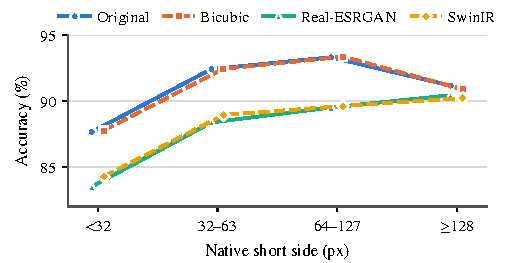
\includegraphics[width=\linewidth]{figures/native_size}
\caption{Same-checkpoint accuracy by native short-side band, pooled over 6 backbones $\times$ 5 folds.}
\label{fig:size}
\end{figure}

\begin{figure}[t]
\centering
\setlength{\tabcolsep}{1.5pt}
\begin{tabular}{cccc}
\scriptsize Original & \scriptsize Bicubic & \scriptsize Real-ESRGAN & \scriptsize SwinIR \\
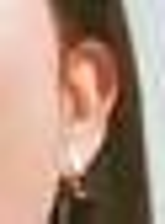
\includegraphics[height=2.1cm]{figures/qual_f_orig} &
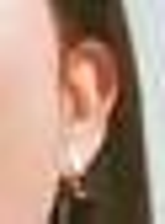
\includegraphics[height=2.1cm]{figures/qual_f_bic} &
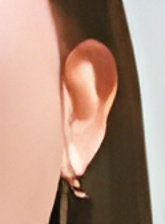
\includegraphics[height=2.1cm]{figures/qual_f_res} &

\includegraphics[height=2.1cm]{figures/qual_f_swin} \\
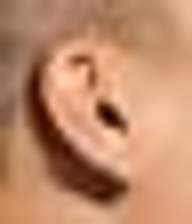
\includegraphics[height=2.1cm]{figures/qual_m_orig} &

\includegraphics[height=2.1cm]{figures/qual_m_bic} &
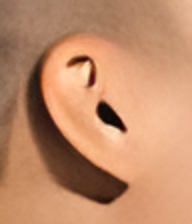
\includegraphics[height=2.1cm]{figures/qual_m_res} &

\includegraphics[height=2.1cm]{figures/qual_m_swin} \\
\end{tabular}
\caption{Recognizer inputs (after the final resize, padding removed) for two crops below 32 pixels that ResNet50 (fold 0) classifies correctly from Original and wrongly from both SR versions. Top: female, $31\times42$ pixels; bottom: male, $24\times28$ pixels. Of the 30 such crops in this fold, 27 are male crops predicted as female.}
\label{fig:qual}
\end{figure}

\subsection{Matched-domain retraining}
Table~\ref{tab:matched} retrains each backbone on each variant from the same ImageNet initialization and locked configuration, tests it on that variant, and reports the per-fold paired gap to the backbone's Original-to-Original run. All 18 gaps lie between $-0.36$ and $+0.85$ points, each is smaller than the cell's cross-fold standard deviation, and no per-cell paired $t$-test is significant after Holm correction; 12 of the 18 are positive. Averaged over backbones per fold, the gap is $+0.06$ points for Bicubic, $+0.38$ for Real-ESRGAN, and $+0.36$ for SwinIR, and a TOST test shows equivalence to Original within $\pm1$ point for both SR methods ($p=0.028$ and $0.004$). Because the locked configuration was selected on Original validation data, any tuning bias favors Original; the SR-trained recognizers match it regardless, so this equivalence is conservative. The same checkpoint, by comparison, lost 3.23 and 2.99 points.

\begin{table}[t]
\centering
\caption{Matched-domain retraining: accuracy gap (pp) vs.\ the backbone's own Original-to-Original run (train and test on the same variant), Protocol B, mean over 5 folds; last row: 95\% CI of the fold-level mean gap.}
\label{tab:matched}
\small
\begin{tabular}{@{}lrrr@{}}
\toprule
Model & Bicubic & Real-ESRGAN & SwinIR \\
\midrule
VGG19            & $-0.33$ & $+0.01$ & $-0.02$ \\
MobileNetV2      & $-0.14$ & $+0.24$ & $+0.71$ \\
ResNet50         & $-0.05$ & $+0.68$ & $+0.14$ \\
EfficientNet-B0  & $-0.36$ & $-0.21$ & $+0.06$ \\
Swin-T           & $+0.61$ & $+0.71$ & $+0.79$ \\
MaxViT-T         & $+0.61$ & $+0.85$ & $+0.47$ \\
\midrule
Mean & $+0.06$ & $+0.38$ & $+0.36$ \\
95\% CI & $[-0.22, 0.33]$ & $[-0.27, 1.03]$ & $[-0.01, 0.73]$ \\
\bottomrule
\end{tabular}
\end{table}

\subsection{Label-free adaptation}\label{sec:adapt}
The same-checkpoint loss can also be reduced without retraining (last rows of Table~\ref{tab:main}; per-backbone values in Supplementary Table~S3). Threshold recalibration cuts it to 1.43 and 1.28 points and restores male recall from 87.9\% to 93.3\% (Original: 94.6\%), which undoes most of the shift toward the female class. AdaBN cuts it to 1.18 and 0.76 points for the BatchNorm backbones, recovering 70\% and 79\% of their loss. Recalibration helps in 53 of 60 backbone-fold-SR cases and AdaBN in 38 of 40, but about one point remains (95\% CIs exclude zero); only retraining closes the gap fully.

\section{Discussion}\label{sec:discussion}
Table~\ref{tab:matched} helps explain the loss. If SR erased gender-discriminative detail, for instance by replacing the ridges and folds of the pinna with generic texture, a recognizer retrained on SR images should still fall short of one trained on Original. It does not: the retrained SR gap is equivalent to zero within one point. The simplest explanation is a distribution shift: the signal the recognizer uses survives SR, but its texture statistics differ from those seen in training. The one-sided recall change in Section~\ref{sec:main} supports this, since a shift that consistently pushes the margin toward one class is what a mismatch in input statistics would produce. Matched-domain parity shows that the signal these recognizers exploit is preserved; it does not show that every fine morphological detail is. The adaptation results give a more direct test: with the weights unchanged, re-aligning only the decision threshold or the normalization statistics recovers most of the loss, which would not be possible if SR had removed the information.

These results give a three-level decision rule for deployment. First, inserting an off-the-shelf SR model before an already-trained classifier costs several points of accuracy, mostly on small crops, and silently changes the operating point, so a threshold tuned on Original inputs no longer holds. Second, if SR must be used and retraining is not possible, recalibrating the threshold or the BatchNorm statistics on unlabeled SR images recovers more than half of the loss at almost no cost. Third, if the classifier can be retrained, SR inputs are as learnable as Original ones, but not better, so training and deploying on Original remains simpler and cheaper.

All experiments use EarVN1.0, which contains 164 subjects from a single (Asian) population, and we did not evaluate on a second dataset. To our knowledge, EarVN1.0 is the largest ear dataset with gender labels, about 28 times larger than AWE (1{,}000 images of 100 subjects)~\cite{emersic2017}. Our findings agree in direction with SwinIR degrading ear identity recognition on UERC~\cite{markicevic2023} and with restoration preprocessing giving little benefit to CNN classifiers~\cite{pei2021}; a cross-dataset test on AWE is the natural next step. We evaluate two SR models with a similar blind, real-world-degradation training philosophy; diffusion-based SR is left open. Every recognizer receives a $224\times224$ input regardless of the upsampling factor, which may cap what SR can contribute. Native aspect ratio and padding fraction differ by sex at the subject level (Mann--Whitney $p<0.01$, rank-biserial effect 0.26), a possible geometric shortcut. A logistic regression on these cues alone, trained and tested on the same subject-disjoint folds, reaches only 55--57\% balanced accuracy, below the 61.8\% majority accuracy and far below the recognizers. Because the padding is identical across the four inputs, it can affect absolute accuracy but cannot explain $\Delta_{\text{SR}}$.

\section{Conclusion}\label{sec:conclusion}
Under a same-checkpoint, subject-disjoint protocol, Real-ESRGAN and SwinIR reduce ear-based gender accuracy on EarVN1.0 for all six backbones, while bicubic upsampling does not. The loss is concentrated in crops below 128 pixels and shifts decisions toward the female class. Retraining on SR images recovers Original accuracy, and label-free recalibration of the threshold or the BatchNorm statistics recovers most of it, which points to a shift in input statistics. Off-the-shelf SR should not be placed before a deployed classifier without at least recalibration; recognition-aware SR is a natural next step.

\begin{thebibliography}{99}
\footnotesize
\setlength{\itemsep}{0pt}
\setlength{\parsep}{0pt}
\setlength{\topsep}{0pt}

\bibitem{nguyenquoc2020}
H. Nguyen-Quoc and V. T. Hoang, ``Gender recognition based on ear images: a comparative experimental study,'' in \emph{Proc. ISRITI}, 2020, pp. 451--456.

\bibitem{hoang2019earvn}
V. T. Hoang, ``EarVN1.0: A new large-scale ear images dataset in the wild,'' \emph{Data in Brief}, vol. 27, 2019, Art. no. 104630.

\bibitem{emersic2017}
Z. Emer\v{s}i\v{c}, V. \v{S}truc, and P. Peer, ``Ear recognition: More than a survey,'' \emph{Neurocomputing}, vol. 255, pp. 26--39, 2017.

\bibitem{pflug2012}
A. Pflug and C. Busch, ``Ear biometrics: a survey of detection, feature extraction and recognition methods,'' \emph{IET Biometrics}, vol. 1, no. 2, pp. 114--129, 2012.

\bibitem{hassaballah2019}
M. Hassaballah, H. A. Alshazly, and A. A. Ali, ``Ear recognition using local binary patterns: A comparative experimental study,'' \emph{Expert Systems with Applications}, vol. 118, pp. 182--200, 2019.

\bibitem{lei2013}
J. Lei, J. Zhou, and M. Abdel-Mottaleb, ``Gender classification using automatically detected and aligned 3D ear range data,'' in \emph{Proc. ICB}, 2013, pp. 1--7.

\bibitem{khorsandi2013}
R. Khorsandi and M. Abdel-Mottaleb, ``Gender classification using 2-D ear images and sparse representation,'' in \emph{Proc. WACV}, 2013, pp. 461--466.

\bibitem{realesrgan}
X. Wang, L. Xie, C. Dong, and Y. Shan, ``Real-ESRGAN: Training real-world blind super-resolution with pure synthetic data,'' in \emph{Proc. ICCV Workshops}, 2021, pp. 1905--1914.

\bibitem{swinir}
J. Liang \emph{et al.}, ``SwinIR: Image restoration using Swin Transformer,'' in \emph{Proc. ICCV Workshops}, 2021, pp. 1833--1844.

\bibitem{vgg}
K. Simonyan and A. Zisserman, ``Very deep convolutional networks for large-scale image recognition,'' in \emph{Proc. ICLR}, 2015.

\bibitem{mobilenetv2}
M. Sandler \emph{et al.}, ``MobileNetV2: Inverted residuals and linear bottlenecks,'' in \emph{Proc. CVPR}, 2018, pp. 4510--4520.

\bibitem{resnet}
K. He \emph{et al.}, ``Deep residual learning for image recognition,'' in \emph{Proc. CVPR}, 2016, pp. 770--778.

\bibitem{efficientnet}
M. Tan and Q. Le, ``EfficientNet: Rethinking model scaling for convolutional neural networks,'' in \emph{Proc. ICML}, 2019, pp. 6105--6114.

\bibitem{maxvit}
Z. Tu \emph{et al.}, ``MaxViT: Multi-axis vision transformer,'' in \emph{Proc. ECCV}, 2022, pp. 459--479.

\bibitem{swintransformer}
Z. Liu \emph{et al.}, ``Swin Transformer: Hierarchical vision transformer using shifted windows,'' in \emph{Proc. ICCV}, 2021, pp. 9992--10002.

\bibitem{dai2016}
D. Dai, Y. Wang, Y. Chen, and L. Van Gool, ``Is image super-resolution helpful for other vision tasks?'' in \emph{Proc. WACV}, 2016, pp. 1--9.

\bibitem{pei2021}
Y. Pei, Y. Huang, Q. Zou, X. Zhang, and S. Wang, ``Effects of image degradation and degradation removal to CNN-based image classification,'' \emph{IEEE Trans. Pattern Anal. Mach. Intell.}, vol. 43, no. 4, pp. 1239--1253, 2021.

\bibitem{grm2020}
K. Grm, W. J. Scheirer, and V. \v{S}truc, ``Face hallucination using cascaded super-resolution and identity priors,'' \emph{IEEE Trans. Image Process.}, vol. 29, pp. 2150--2165, 2020.

\bibitem{saerens2002}
M. Saerens, P. Latinne, and C. Decaestecker, ``Adjusting the outputs of a classifier to new a priori probabilities: A simple procedure,'' \emph{Neural Comput.}, vol. 14, no. 1, pp. 21--41, 2002.

\bibitem{li2018adabn}
Y. Li, N. Wang, J. Shi, X. Hou, and J. Liu, ``Adaptive batch normalization for practical domain adaptation,'' \emph{Pattern Recognit.}, vol. 80, pp. 109--117, 2018.

\bibitem{markicevic2023}
L. Marki\v{c}evi\'{c}, P. Peer, and \v{Z}. Emer\v{s}i\v{c}, ``Improving Ear Recognition with Super-resolution,'' in \emph{Proc. Int. Conf. on Systems, Signals and Image Processing (IWSSIP)}, 2023, pp. 1--5.

\end{thebibliography}

\end{document}
